\documentclass[11pt]{article}
\usepackage{amsmath, amssymb}
\usepackage{geometry}
\geometry{margin=1in}
\usepackage{fancyhdr}
\usepackage{lastpage}
\usepackage{parskip} % Better paragraph spacing
\usepackage{titlesec} % Better section formatting
\usepackage{graphicx}
\usepackage{float}
\usepackage[most]{tcolorbox}
\usepackage{lmodern}
\usepackage{caption}
\usepackage{hyperref}
\usepackage{listings}
\usepackage{xcolor}

\definecolor{codegreen}{rgb}{0,0.6,0}
\definecolor{codegray}{rgb}{0.5,0.5,0.5}
\definecolor{codepurple}{rgb}{0.58,0,0.82}
\definecolor{backcolour}{rgb}{0.95,0.95,0.92}

% Define code styling
\lstdefinestyle{mystyle}{
    backgroundcolor=\color{backcolour},
    commentstyle=\color{codegreen},
    keywordstyle=\color{magenta},
    numberstyle=\tiny\color{codegray},
    stringstyle=\color{codepurple},
    basicstyle=\ttfamily\footnotesize,
    breakatwhitespace=false,
    breaklines=true,
    captionpos=b,
    keepspaces=true,
    numbers=left,
    numbersep=5pt,
    showspaces=false,
    showstringspaces=false,
    showtabs=false,
    tabsize=2
}

\lstset{style=mystyle}

% Define commands for reusable content
\newcommand{\coursename}{COM-407 Advanced Networks}
\newcommand{\lecturenum}{14}
\newcommand{\lecturedate}{\today}
\newcommand{\professor}{Pavlos Nikoupoulos}

\hypersetup{colorlinks=true,linkcolor=blue,urlcolor=blue}

% Configure section spacing
\titlespacing*{\section}{0pt}{2ex plus 1ex minus .2ex}{1.5ex plus .2ex}
\titlespacing*{\subsection}{0pt}{1.5ex plus 1ex minus .2ex}{1ex plus .2ex}
% Header / Footer
\pagestyle{fancy}
\fancyhf{}
\fancyhead[L]{\coursename}
\fancyhead[R]{Lecture \lecturenum}
\fancyfoot[L]{EPFL - Computer Science}
\fancyfoot[C]{Author: Jonathan Dutoit}
\fancyfoot[R]{Page \thepage\ of \pageref{LastPage}}

\begin{document}

\begin{center}
  {\large EPFL - Computer Science} \\[0.5em]
  {\Large \textbf{\coursename}} \\[0.5em]
  {\large Lecture \lecturenum\ --- \lecturedate} \\[0.5em]
  {\large Author: Jonathan Dutoit} \\[0.5em]
  {\large Professor: \professor} \\[0.5em]
\end{center}

\vspace{2cm}

\begin{center}
  {\LARGE \textbf{External Routing}} \\
  BGP
\end{center}

\vspace{1cm}

\section*{1. How does BGP work?}

\begin{itemize}
	\item BGP routers/\textit{\textcolor{green}{speakers}} talk to each other \textit{\textcolor{green}{over TCP}} connections
	\item Each BGP router [BGP-4, RFC 4271]:
		\begin{itemize}
			\item receives and stores \textit{\textcolor{red}{candidate routers}} from its BGP neighbors, after applying \textit{\textcolor{blue}{import}} policy rules
			\item applies the \textit{\textcolor{blue}{decision process}} to \textit{\textcolor{red}{select at most one route}} per destination prefix and keeps all other imported routers as \textcolor{blue}{backup}
	\item exports the \textit{\textcolor{red}{selected}} routes to BGP neighbors, after applying \textit{\textcolor{blue}{export}} policy rules and possibly \textit{\textcolor{blue}{aggregation}}
		\end{itemize}
	\item Routers are advertised via \textbf{UPDATE} messages that contain \textit{\textcolor{blue}{only modifications = }} \textbf{new paths, withdrawals}
	\item Other messages: \textbf{OPEN} (=sync after boot-up), \textbf{NOTIFICATION} (= reset), \textbf{KEEPALIVE} (= periodic beacon to notify BGP peers that BGP on router is running); absence of KEEPALIVE after some time triggers a withdrawal UPDATE
\end{itemize}

\section*{2. Types of BGP (used in parallel)}


\begin{minipage}{0.6\textwidth}
\begin{itemize}
	\item \textcolor{red}{e}(xternal)\textcolor{red}{-BGP}:
		\begin{itemize}
			\item routing exchange between routers in \textit{\textcolor{blue}{different}} domains (i.e border routers across neighbor domains)
		\end{itemize}
	\item \textcolor{red}{i}(nternal)\textcolor{red}{-BGP}: 
		\begin{itemize}
			\item routing exchange between routers \textit{\textcolor{blue}{within}} same domain (i.e. domain's border or other internal BGP-speaking routers)
		\end{itemize}
\end{itemize}
In i-BGP, BGP \textcolor{blue}{speakers/peers:}
\begin{itemize}
	\item form a \textcolor{purple}{BGP mesh} network (all-to-all)
	\item advertize routes learn from e-BGP but they \textcolor{red}{never}:
		\begin{itemize}
			\item repeat routes learnt from i-BGP to avoid redundant traffic
			\item prepend own AS number over i-BGP
			\item modify the "NEXT-HOP" attribute of a route
		\end{itemize}
	\item know about inter-domain link subnets via IGP
\end{itemize}

\end{minipage}
\hfill
\begin{minipage}{0.4\textwidth}
\centering
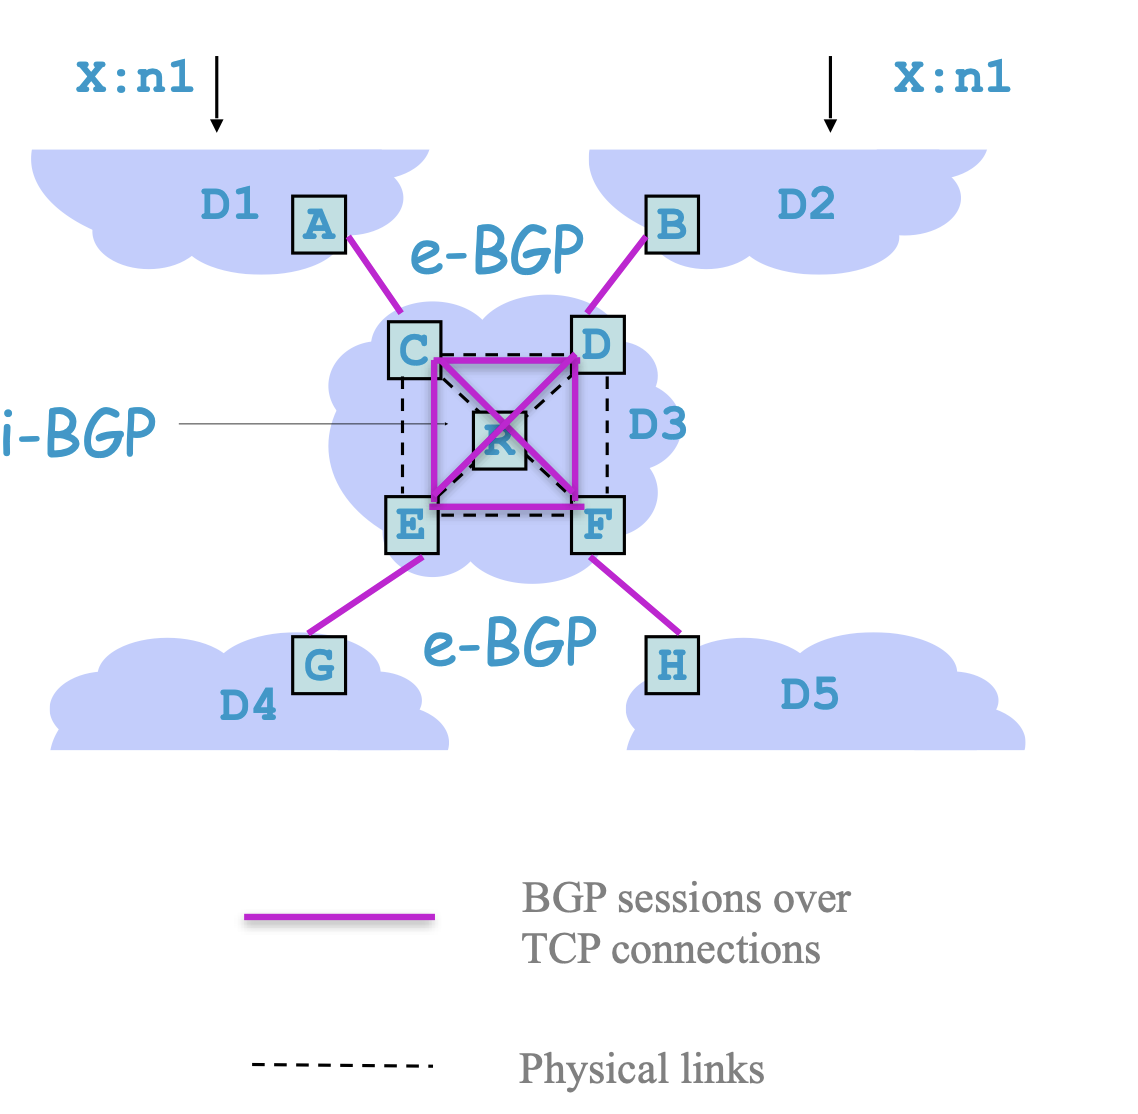
\includegraphics[width=\linewidth]{bgp}
\end{minipage}
\begin{tcolorbox}[
  colback=gray!15,     % background color
  colframe=black!50,    % border color
  boxrule=1pt,       % border thickness
  arc=3mm,             % rounded corners
  left=4mm, right=4mm, top=2mm, bottom=2mm % padding
]
\textbf{Say what is always true}

1. Two BGP peers must be connected by a TCP connection. \\
2. Two BGP peers must be "on link" (on the same subnet) \\

\vspace{0.2cm}
A. 1 \\
B. 2 \\
C. 1 and 2 \\
D. None \\
E. I don't know \\

\textbf{Answer}: A. Internal peers need not be "on link". BGP peers communicate (typically) with TCP. 
\end{tcolorbox}

\begin{tcolorbox}[
  colback=gray!15,     % background color
  colframe=black!50,    % border color
  boxrule=1pt,       % border thickness
  arc=3mm,             % rounded corners
  left=4mm, right=4mm, top=2mm, bottom=2mm % padding
]
\textbf{Which BGP updates may be sent?}

\begin{minipage}{0.6\textwidth}
1. C $\Rightarrow$ A AS-PATH = [D3 D2 X : n1] \\
2. D $\Rightarrow$ E AS-PATH [D2 X : n1] \\
3. C $\Rightarrow$ E AS-PATH = [D2 X : n1]

\end{minipage}
\hfill
\begin{minipage}{0.3\textwidth}
\centering
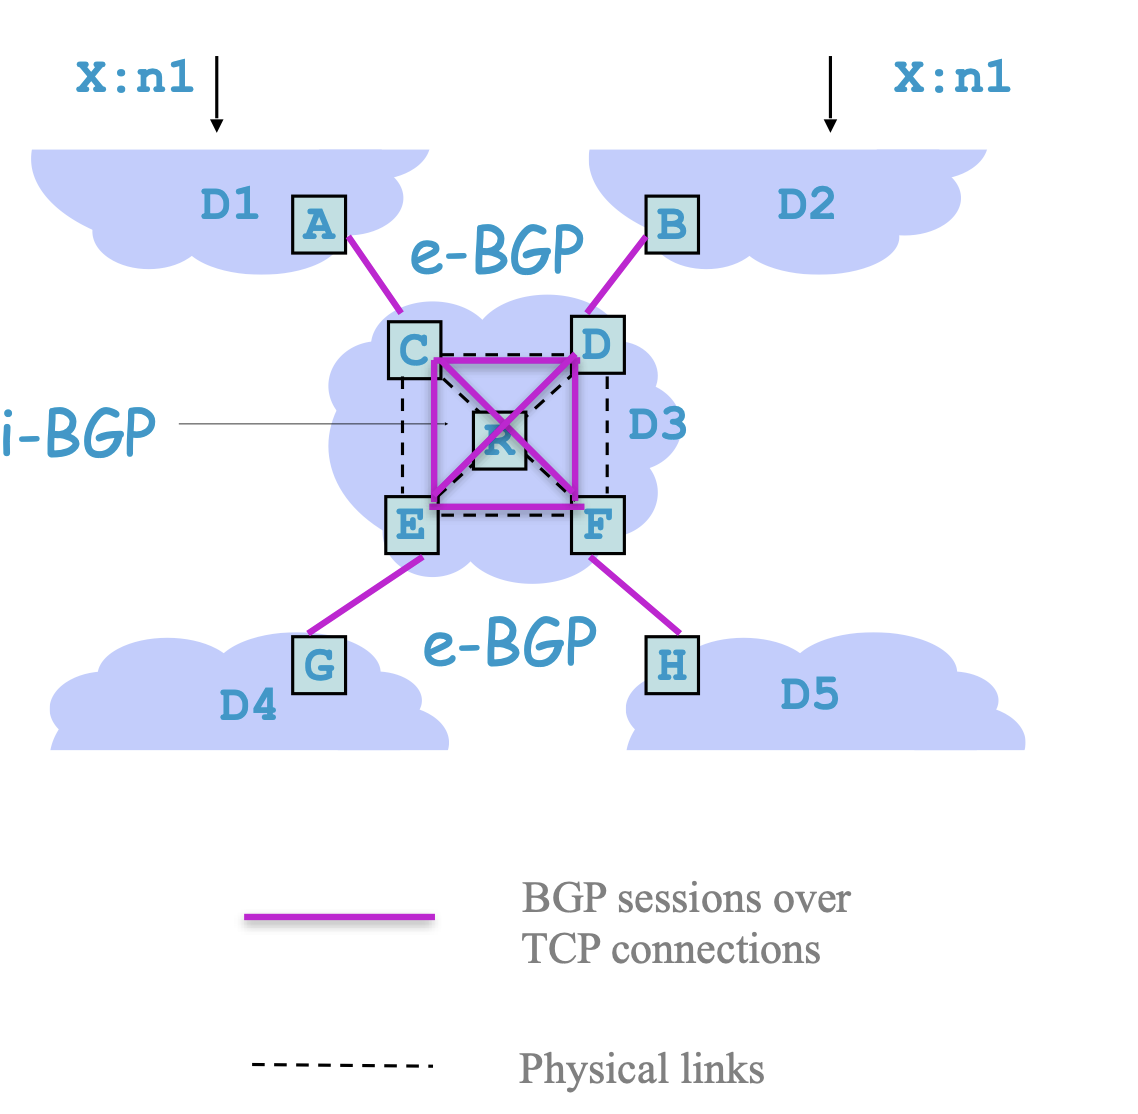
\includegraphics[width=\linewidth]{bgp}
\end{minipage}

A. 1 \\
B. 2 \\
C. 3 \\ 
D. 1 and 2 \\
E. 1 and 3 \\
F. 2 and 3 \\
G. All \\ 
H. None \\ 
I. I don't know \\ 

\textbf{Answer}: D. The router C $\Rightarrow$ E was learnt via internal BGP. Therefore, it should \textit{\textcolor{red}{not be re-advertized}} over i-BGP. 
\end{tcolorbox}

\section*{Operation of a BGP router}
% Quick centered image
\begin{figure}[H]
    \centering
    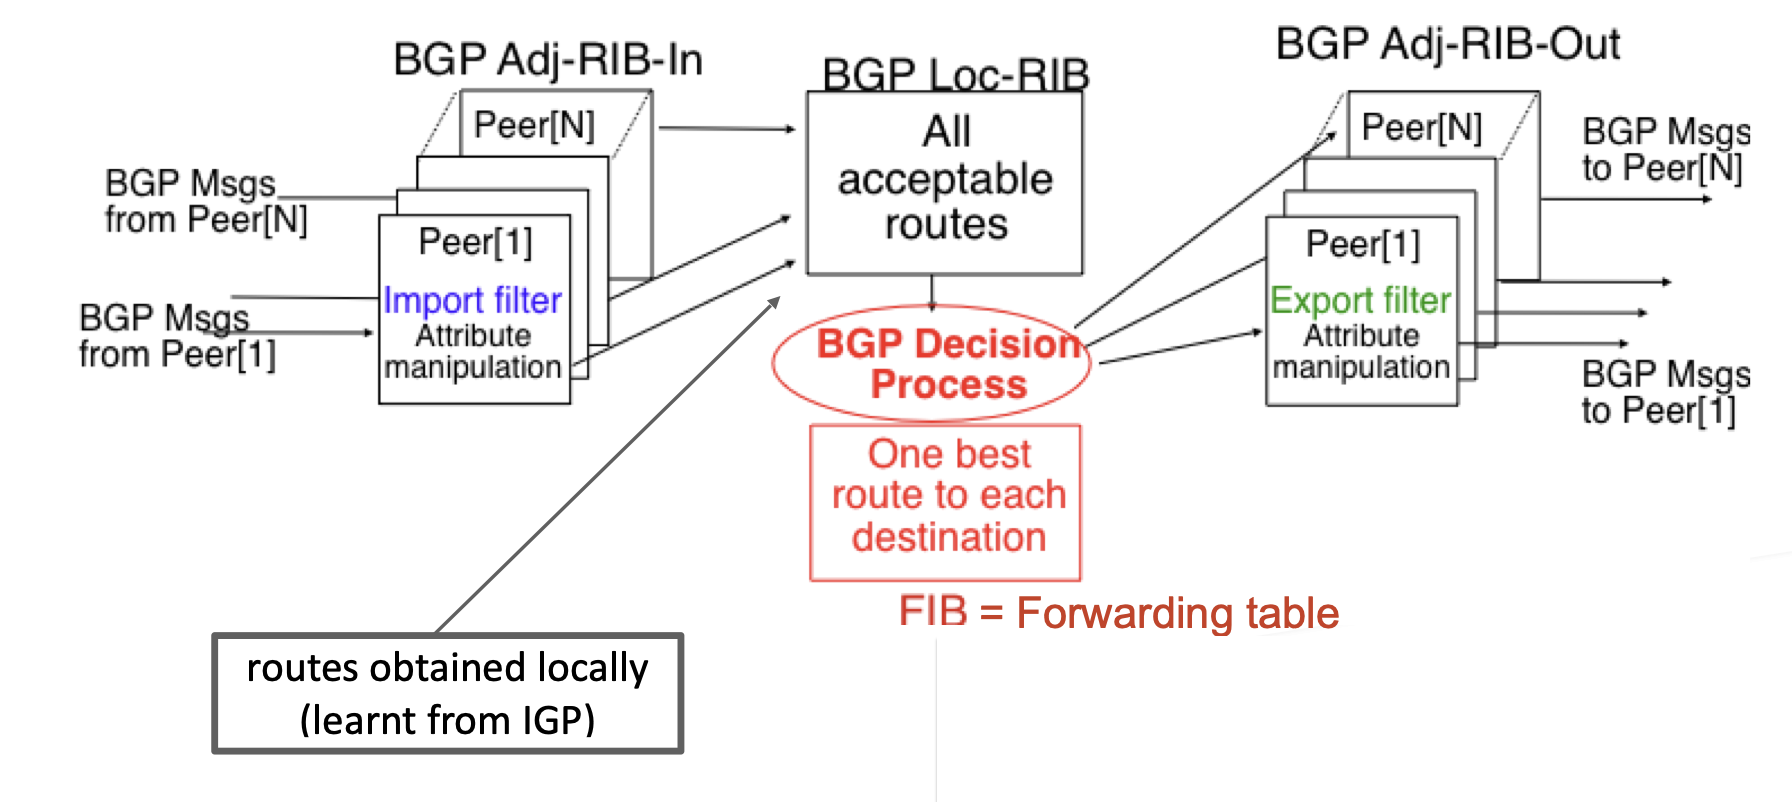
\includegraphics[width=0.8\textwidth]{decision-process}
    \label{fig:LABEL}
\end{figure}

RIB - Route Information base, \\
IGP - Internal Gateway Protocol

\newpage

\section*{Routes, RIBs, Routing Table}

\begin{minipage}{0.6\textwidth}
An advertised \textit{\textcolor{red}{route}} has several attributes:
\begin{itemize}
	\item \textbf{destination} (subnet) prefix
	\item \textbf{path} to destination 
	\item \textbf{NEXT-HOP} (modified by e-BGP, left unchanged by i-BGP
	\item \textbf{ORIGIN}: route learnt from IGP, BGP, static
	\item Other attributes...
\end{itemize}

\end{minipage}
\begin{minipage}{0.4\textwidth}
\centering
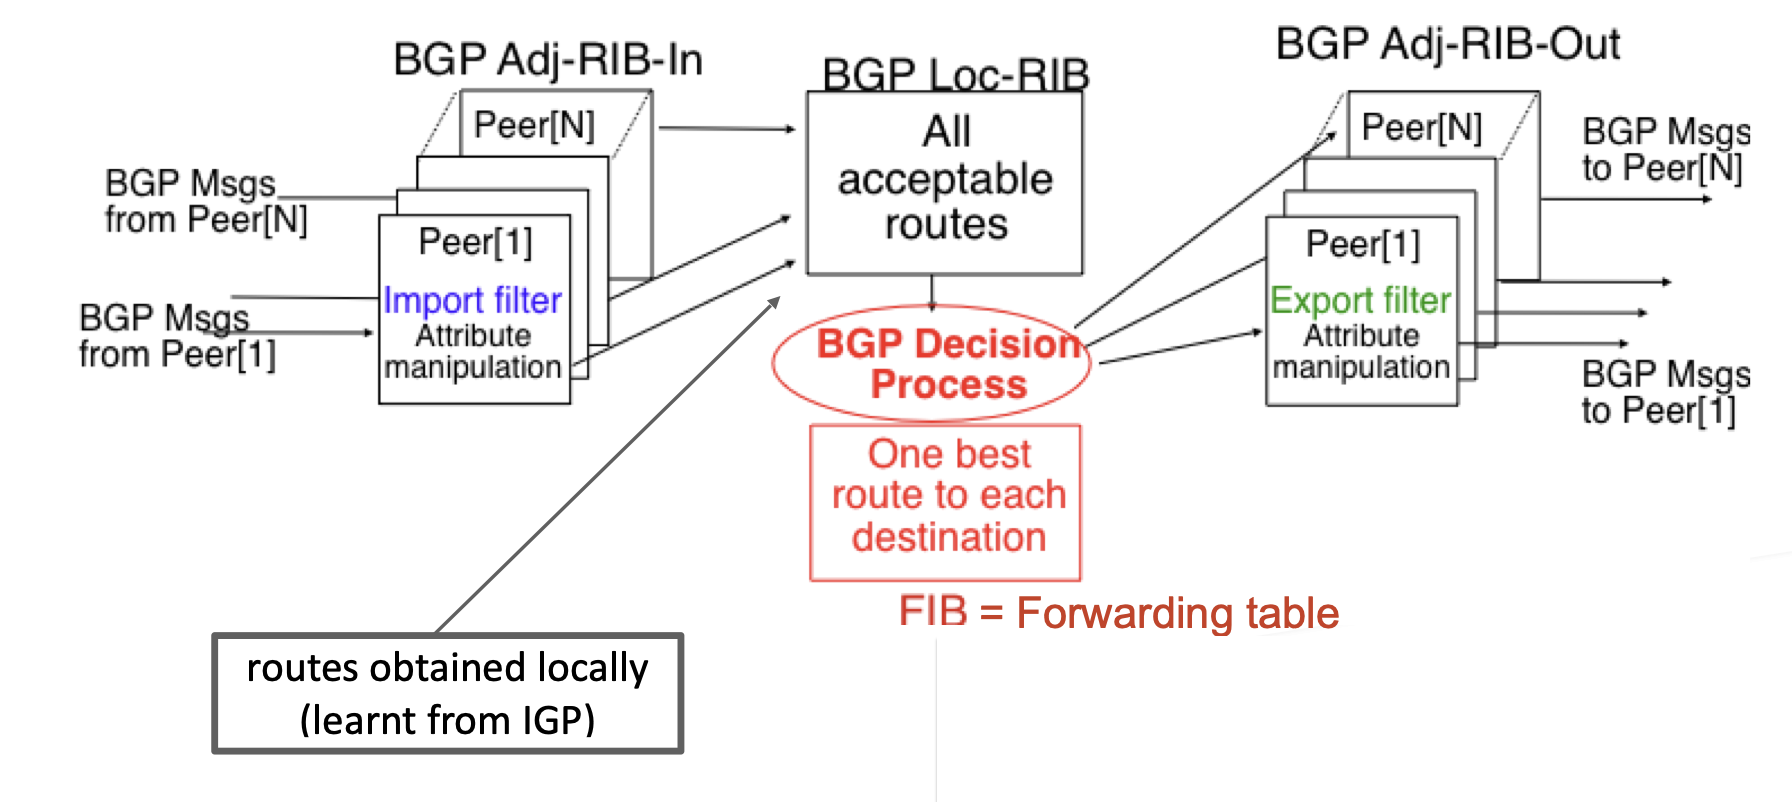
\includegraphics[width=\linewidth]{decision-process}
\end{minipage}

\vspace{0.3cm}
Routers + their attributes are stored in the \textcolor{blue}{Routing Information Bases (RIBs):} 
\begin{center}
\textbf{Ajd-RIB-in, Loc-RIB, Adj-RIB-out}
\end{center}

Like any IP host or router, a BGP router also has an IP \textcolor{red}{Forwarding Table} used for packet forwarding, in real time

\section*{The Decision Process}
The decision process chooses \textcolor{red}{\textit{at most one route}} to \textcolor{red}{each} different destination \textit{\textcolor{red}{prefix}} as best 

\textit{\textcolor{red}{How?}}
\begin{itemize}
	\item A route can be selected only if its next-hop is \textcolor{blue}{reachable}
	\item For each dest prefix, all acceptable routes are compared w.r.t. their \textcolor{blue}{attributes} using a \textcolor{blue}{sequence of criteria} (until only one route remains); a typical sequence is: \\
		0. Highest weight (cisco proprietary) \\
		1. Highest LOCAL-PREF \\
		2. Shortest AS-PATH \\
		3. Lowest MED (multi-exit discriminator), if taken seriously this domain \\ 
		4. e-BGP $>$ i-BGP \\
		5. Shortest path to NEXT-HOP, according to IGP \\
		6. Lowest BGP identifier 
	\item The result of the decision process is stored in forwarding talbe and in Adj-RIB-out (at most \textcolor{red}{\textit{one route per destination per BGP peer}})
	\item The router sends updates when Adj-RIB-out \textit{\textcolor{blue}{changes}} (addition or withdrawal) after applying \textit{\textcolor{blue}{export rules}}
\end{itemize}

\section*{Fundamental Example}
\begin{minipage}{0.6\textwidth}
\begin{itemize}
	\item 4 BGP routers connected directly (solid lines) or indirectly (dash lines), speaking both e-BGP and i-BGP; 
	\item 2 Ases, \textbf{x} and \textbf{y}, each one running its own IGP.
	\item Assume R3 and R4 are configured to advertize \textcolor{red}{both} prefixes of \textbf{y}. 
\end{itemize}

\textbf{\textcolor{blue}{We focus on R1 and show its BGP information bases}}

\end{minipage}
\hfill
\begin{minipage}{0.4\textwidth}
\centering
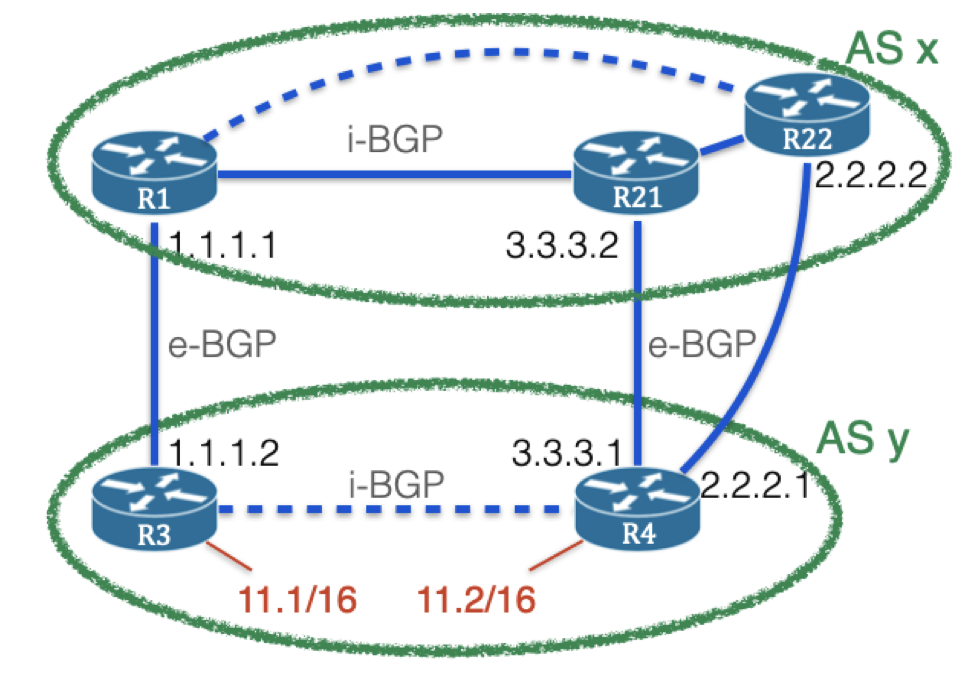
\includegraphics[width=\linewidth]{another-fundamental-example}
\end{minipage}
\section*{Another Fundamental Example}
\begin{itemize}
	\item 3 BGP routers in AS \textbf{x}, also running an OSPF
	\item Assume:
		\begin{itemize}
			\item all link costs are equal to 1. 
			\itrm R3 and R4 advertize \textcolor{red}{\textit{only}} their directly attached prefixes. 
		\end{itemize}
\end{itemize}

\vspace{0.3cm}
\textbf{\textcolor{blue}{We focus on R1 and show it's BGP information bases}}


\section*{How are routers originated (=sourced)?}

Several methods for sourcing a route:
\begin{itemize}
	\item \textcolor{blue}{Static configuration}: \textcolor{red}{manually} tell this BGP router which prefixes to originate ("network"command in FRR)
	\item \textcolor{blue}{Redistribute connected}: tell this BGP router to originate \textit{\textcolor{red}{all directly attached prefixes}} (all routers in network may run i-BGP, no need for IGP in this case)
	\item \textcolor{blue}{Redistribute from IGP}: tell this BGP router to originate \textcolor{red}{\textit{all prefixes learnt by IGP}}, e.g.: redistribute OSPF into BGP
		\begin{itemize}
			\item if IGP=OSPF, in principle, \textcolor{red}{\textit{only internal prefixes}} should be redistributed
			\item Such BGP routes have attribute \textcolor{red}{ORIGIN=IGP}
			\item When originated, the BGP NEXT-HOP of such a route is its \textcolor{red}{IGP next-hop}.
		\end{itemize}
\end{itemize}

\textbf{Redistribution} means that we redistribute information learn by BGP to IGP and from IGP to BGP! 

\section*{2. Aggregation (of routes)}

Routes usually \textcolor{red}{\textit{overlap}}

\begin{itemize}
	\item expected very frequently in IPv6 (recall the way we delegate prefixes),
	\item less frequently in IPv4
\end{itemize}

So, \textit{\textcolor{blue}{prefix aggregation}} can reduce the number of routes
\begin{itemize}
	\item In IP forwarding tables
	\item In BGP advertisements
\end{itemize}

Otherwise several hundreds of thousands of entries or advertizements (e.g., consider transit ISPs that rarely have a default route to 0.0.0.0)

\begin{tcolorbox}[
  colback=gray!15,     % background color
  colframe=black!50,    % border color
  boxrule=1pt,       % border thickness
  arc=3mm,             % rounded corners
  left=4mm, right=4mm, top=2mm, bottom=2mm % padding
]
\textbf{Can AS3 aggregate these routes into a single one?}

% Quick centered image
\begin{figure}[H]
    \centering
    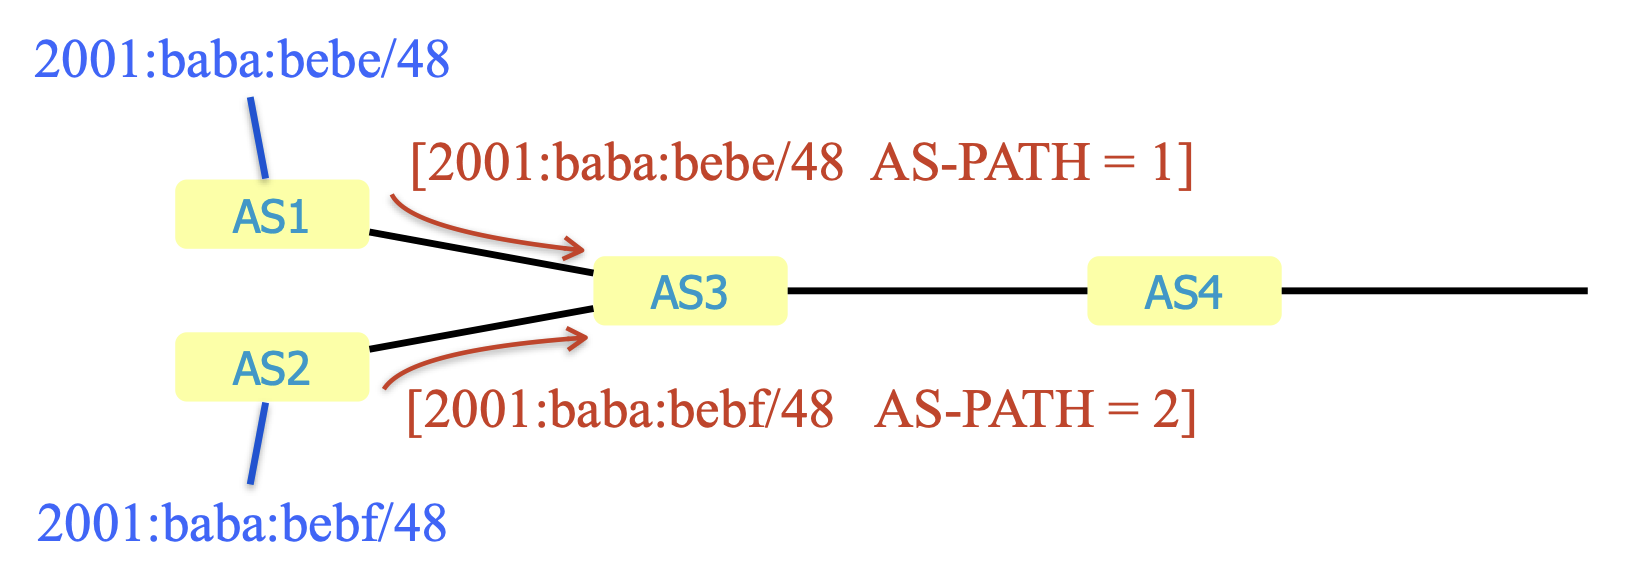
\includegraphics[width=0.8\textwidth]{aggregate}
    \label{fig:LABEL}
\end{figure}

\vspace{0.3cm}
A. Yes and the aggregated prefix is 2001:baba:bebe/47 \\
B. Yes and the aggregated prefix is 2001:baba:bebf/48 \\
C. Yes but the aggregated prefix is none of the above \\
D. No \\
E. I don't know \\
\textbf{Answer}: A. The two prefixes are contiguous and ca be aggregatedas 2001:baba:bebe/47
\end{tcolorbox}

\section*{3. How routes learnt by BGP are written into Forwarding Tables?}

Two ways: \\

1. \textcolor{red}{\textit{Redistribution of BGP into IGP}}: route learnt by BGP is \textcolor{blue}{passed to IGP} (e.g., OSPF)
\begin{itemize}
	\item Typically \textcolor{blue}{only} routers learnt by \textcolor{blue}{e-BGP} are redistributed (unless BGP redistribute-internal is used)
	\item IGP propagates routing information to all routers within domain
	\item Works with OSPF, might not work with other IGPs (tables too large for IGP)
\end{itemize}

2. \textcolor{red}{Injection} \textbf{Destination Prefix and NEXT-HOP of BGP route is \textcolor{blue}{directly copied} into forwarding table}
\begin{itemize}
	\item \textcolor{red}{Why} used? IGP avoids dealing with a large number of table entries (consider convergence issues in distance-vector algorithms, such as RIP).
	\item Injection helps only the particular BGP router; Routing information is not propagated to other intra-domain routers. 
	\item Typically used in Cisco routers and FRR. 
\end{itemize}

\section*{Example (re-distribution)}

\section*{Example (injection)}

\section*{Final Exam}

The last exam is going to be related to the last years. 

Upload 2 different versions: a blank and one with solutions. Start with the blank one is \textbf{super important!}

Need to practice to finish the exam on time. The course is "easy", but the examen can only be finished with practice.

There will be a cheatsheet 3 A4 sheets (6 pages). Slides authorized, everything!

Q&A session in the last week. Tuesday is a good time, maybe wednesday morning.  

\end{document}
